\section{Environment Models}
Within this work, we will encounter several different regions of the space environment -- This section provides a collected overview of each region and the models used.
\subsection{Magnetic Field}
\paragraph{Magnetic Dipole}
\label{section:dipole_model}
To first order, the Earth's magnetic field can be approximated as a dipole, with origin at the Earth's center, and a tilt of $\approx 11^\circ$ from the axis of rotation. The dipole model, sometimes referred to as the ``centered dipole'' or ``tilted dipole'', is reasonably accurate for midlatitude field measurements over the continental United States, but can deviate significantly from the true field elsewhere. Similarly, the dipole field model is reasonably accurate for middle latitudes, below $\approx$ 10 Earth radii, but become increasingly inaccurate at higher latitudes, and at larger distances from the Earth, where the Earth's internal field is no longer dominant.

The dipole model, however, excels in its simplicity -- the dipole magnetic field can be completely described in a closed form, and can be computed rapidly and reliably.

The dipole potential is given by:
\begin{equation}
\psi_{dip} = B_0\big(\frac{R_e}{r}\big)^2\cos\theta
\end{equation}

The individual components of the magnetic field are given by the negative gradient of the scalar potential:

\begin{eqnarray}
& \vec{B} = -\nabla \psi \\
& B_r = -2 B_0\big(\frac{R_e}{r}\big)^3\cos\theta \\
& B_{\theta} = -B_0\big(\frac{R_e}{r}\big)^3 \sin\theta \\ 
& B_\phi = 0
\end{eqnarray}

Within this work we use $B_0 = 31.5$ $\mu$T and $R_e=6371$ km.

A single fieldline, determined by integrating the direction of the field vector, can be described by it's \emph{L-shell} -- the fieldline's altitude, in units of Earth radii, measured at the equator. 

For the dipole field, the radius of a field line at any latitude is related by:
\begin{equation}
R(\lambda) = R_e L \cos^2 \lambda
\end{equation}


The dipole field can then be used as an orthogonal coordinate system, with any location being specified by a latitude, longitude, and L-shell \citep{McIlwain1961}. 
\paragraph{IGRF}

The International Geomagnetic Reference Field (IGRF) is a 13th-order spherical expansion model, with coefficients updated every few years based on terrestrial measurements \citep{Thebault2015}. Within this work we use the IGRF-12 model as a realistic representation of the Earth's internal magnetic field.

IGRF is quick and simple to calculate at any given location, and is much closer to reality than a simple dipole field. However, due to the added complexity, there are not closed-form expressions for field line trajectories or L-shells, which can make dealing with IGRF (and any higher-order model) more cumbersome.

\paragraph{Tsyganenko Corrections}
The dipole and IGRF models represent the Earth's internally-generated magnetic field. However, as one moves further away from the Earth ($L > \approx 8$), the Earth's internal field becomes less dominant, and external fields, namely forcing from the solar wind, cannot be ignored. The total field present in the space environment is the sum of both internal and external contributions.

Numerous models of the external field exist; within this work we consider the T05 external field model \citep{Tsyganenko2005}. The external field model exhibits seasonal and daily variation. However, for fieldlines below L $\approx$ 7, the external field effects are negligible. 

Figure \ref{fig:fieldline_example} contrasts the dipole, IGRF, and T05-corrected models in the meridional plane; figure \ref{fig:Lshell_example} illustrates the deviation in fieldline contours along the Earth's surface between the dipole and IGRF models.

\begin{figure}[h]
\begin{center}
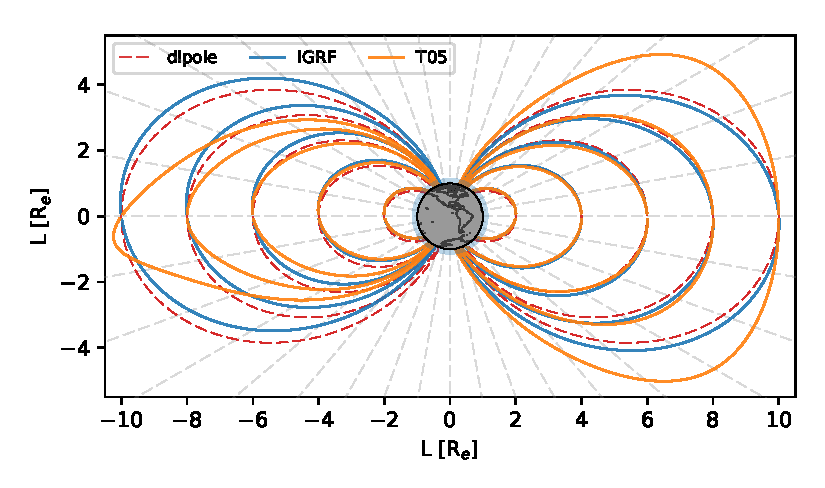
\includegraphics{figures/fieldline_models.pdf}
\end{center}

\caption[Magnetic field models]{Three different magnetic field models, shown in the meridional plane, in geomagnetic coordinates: the tilted dipole, the IGRF model, and the Tsyganenko-Corrected IGRF model. Solar wind is incident on the right side.}
\label{fig:fieldline_example}
\end{figure}
\begin{figure}[h]
\begin{center}
	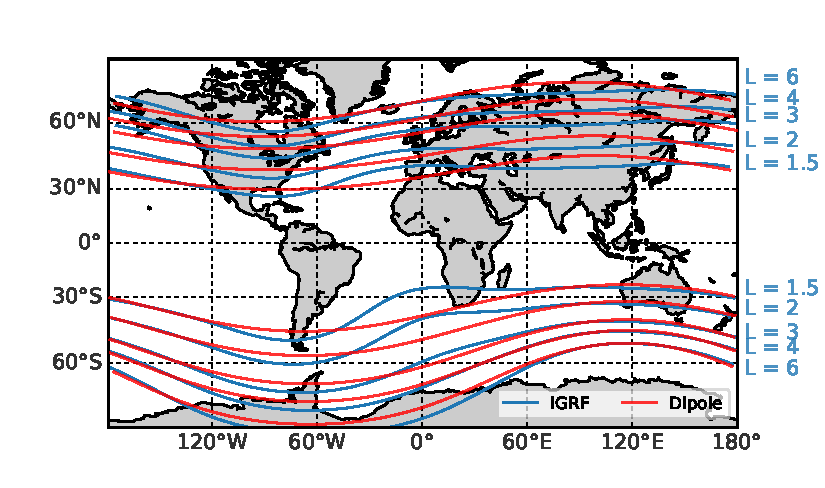
\includegraphics{figures/Lshell_contours.pdf}
\end{center}
\caption[L-shell contours on the Earth's surface]{Fieldline contours along the Earth's surface, shown for the dipole and IGRF models.}
\label{fig:Lshell_example}
\end{figure}


\subsection{Plasmasphere}
The plasmasphere is a region of the space environment surrounding the Earth, and a primary unknown within our modeling. The plasmasphere extends from an altitude of ~1000km up to several Earth radii; typically it is divided into two separate regions: a dense, relatively cold \emph{inner plasmasphere}, and a sparse, relatively hot \emph{outer plasmasphere} or \emph{trough}. The transition boundary between the two regions is a sharp dropoff in plasma density called the \emph{plasmapause}.

Much like the ionosphere, the plasmasphere is a highly variable region, depending on solar conditions ($K_p$), location (latitude, longitude, field line), and time of day (MLT). The large spatial scales, high variability, and sparse availability of in-situ measurements require us to turn to empirical models of each region. We consider three primary models of electron density, and two of electron temperature.

\subsubsection{Overview of Plasmasphere Density Models}

\paragraph{Ngo Model}

The Ngo model is a legacy model used extensively in research at Stanford from the early 1980s through the mid-2000s, notably by \cite{Lauben1998} and \cite{Bortnik2005}, and has heritage dating back to the early days of radioscience at Stanford \citep{Kimura1966} The model uses a Diffusive Equilibrium (DE) model for the inner and outer plasmasphere, onto which the \cite{Carpenter1992} inner plasmasphere model is overlaid. This model was integrated into the legacy Stanford VLF raytracing code, and provided several adjustable parameters, including plasmapause location, constituent ratios, and the ability to include ducts.

\paragraph{Global Core Plasmasphere Model}

The Global Core Plasmasphere Model (GCPM), initially developed in 2000 by \cite{Gallagher1999} with significant updates through the following decade, smoothly transitions between several regional models to provide a continuous model of the plasmasphere. Within this work we use version 2.4, which was released in 2009 and made available by the Space Plasma Physics group at the NASA Marshall Space Flight Center (https://plasmasphere.nasa.gov). GCPM incorporates the \cite{Carpenter1992} inner plasmasphere model and the \cite{Gallagher1995} outer plasmasphere model, with an empirical fit of the plasmapause location between. The polar cap model is derived from \cite{Persoon1983} and \cite{Chandler1991}. All models are connected smoothly to the IRI model of the ionosphere at lower altitudes. The combined GCPM model is parameterized by $K_p$ and MLT.

\paragraph{Simplified GCPM}

GCPM aims to provide a dynamic, complete picture of the plasmasphere as a function of time and $K_p$; however for our purposes GCPM provides too much variation. Additionally, the combination and smoothing between many models is computationally slow. In order to provide quicker computation and to reduce the number of parameters to adjust, we have implemented a simplified version of GCPM.

This model uses the equatorial-plane GCPM model, including the plasmapause location. However we omit any variation in electron density along latitude, and assume densities are constant along each field line. As our region of interest lies primarily within low and mid latitudes, we omit the polar cap model altogether and simply merge the ionosphere into the equatorial trough model. Finally to simplify computation, we model the ionosphere using an empirical fit to IRI -- one for noon, and one for midnight, with a smooth transition along longitude.

Figure \ref{fig:plasma_model_comparison} shows a side-by-side comparison of the three models.
\begin{figure}[h]
\begin{center}
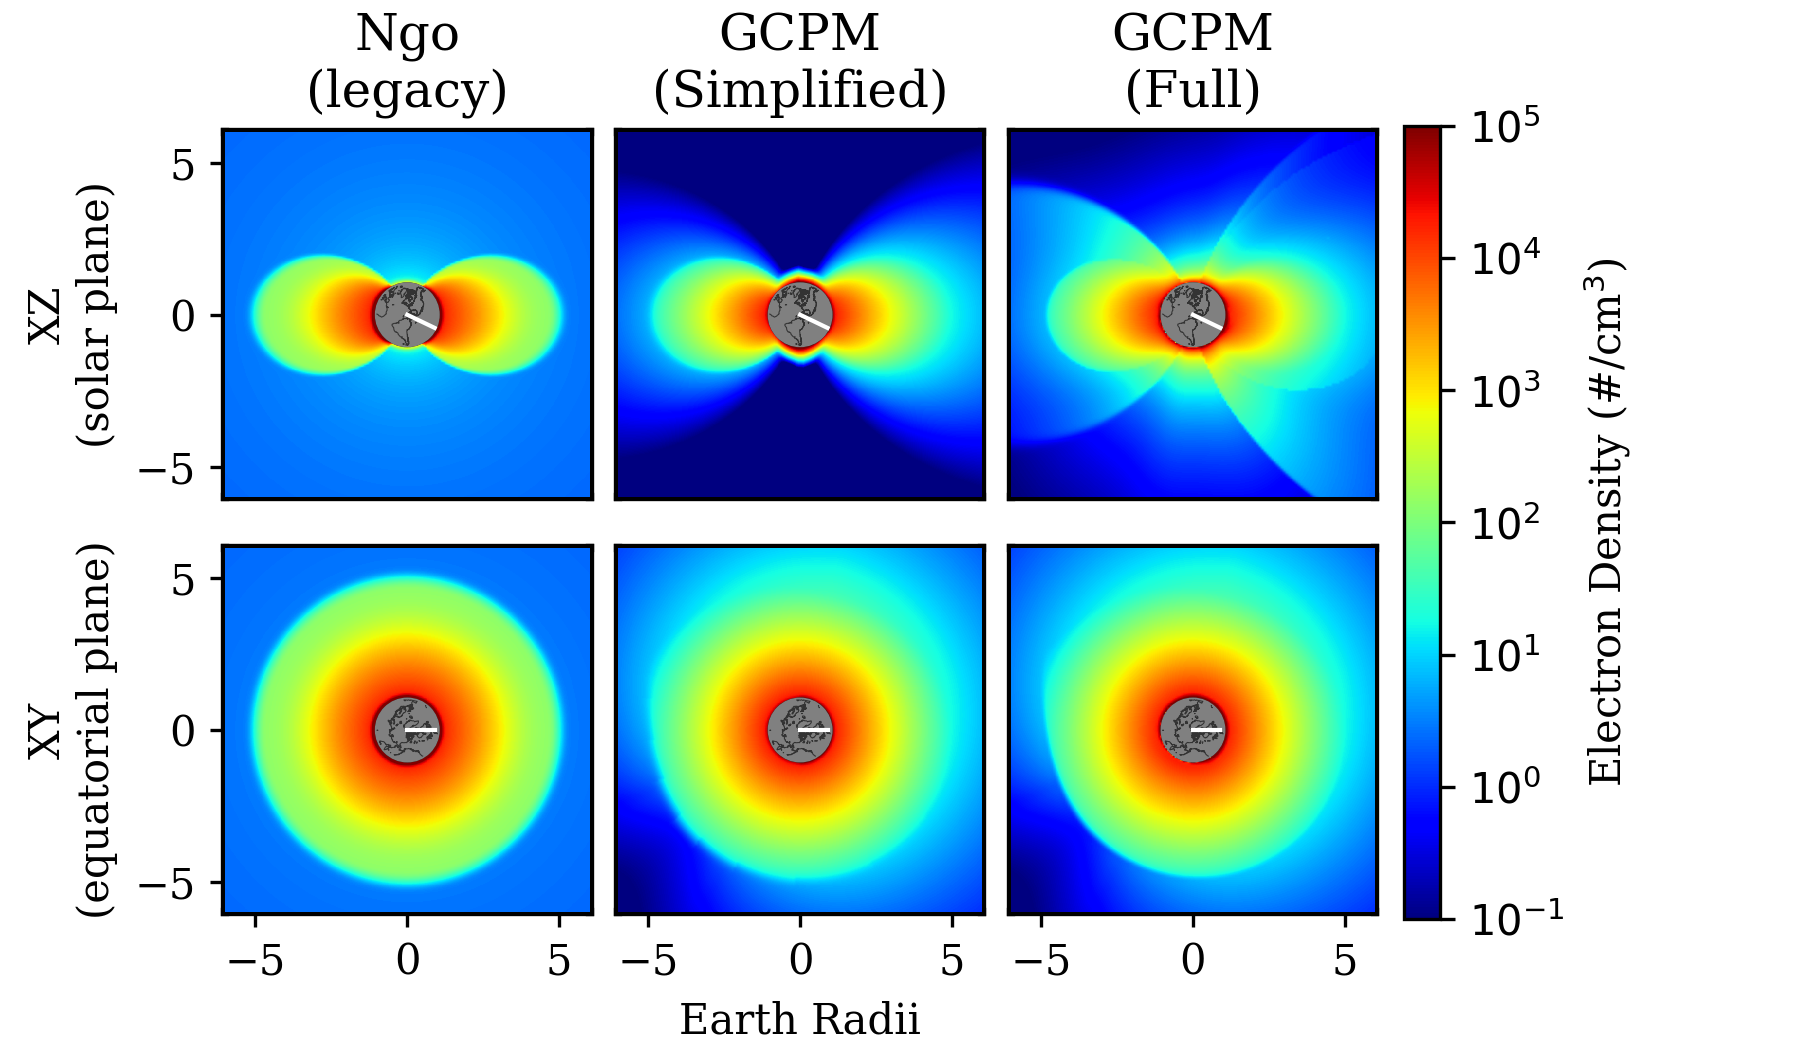
\includegraphics{figures/plasma_model_comparison_serif.png}
\caption[A Comparison of three plasmasphere electron density models]{A comparison of three plasmasphere models: Ngo, simplified GCPM, and full GCPM, for a relatively quiet plasmasphere ($K_p=2$). The top row shows electron density in-plane with the direction of solar influx; the bottom row shows a top down (equatorial cross-section) view. The white line indicates the solar axis. Only electron density is shown, as additional plasma constituents are derived from electron density.}
\label{fig:plasma_model_comparison}
\end{center}
\end{figure}

\subsection{Ionosphere}
The ionosphere, extending from $\approx$ 85 km to 1000 km, is the highly-variable transition region between the terrestrial neutral atmosphere and the sparse plasmas of the space environment. In general, our treatment of wave propagation in the ionosphere is abstracted using the method described in section \ref{section:trans_ionosphere_atten}. However, in raytracing through the plasmasphere, we require a smoothly-varying transition between the plasmasphere and ionosphere models.

\paragraph{IRI}
The International Reference Ionosphere (IRI) is a standard model of several key plasma parameters -- electron density, electron and ion temperatures, ion composition, and so forth. IRI provides detailed outputs as a function of location, altitude, and local time. The GCPM plasma model uses the IRI-2007 implementation \citep{Bilitza2008}; the simplified IRI model is derived from the IRI-2016 model (the most-current available version at time of writing).

\paragraph{Simplified IRI}
\begin{figure}[h]
\begin{center}
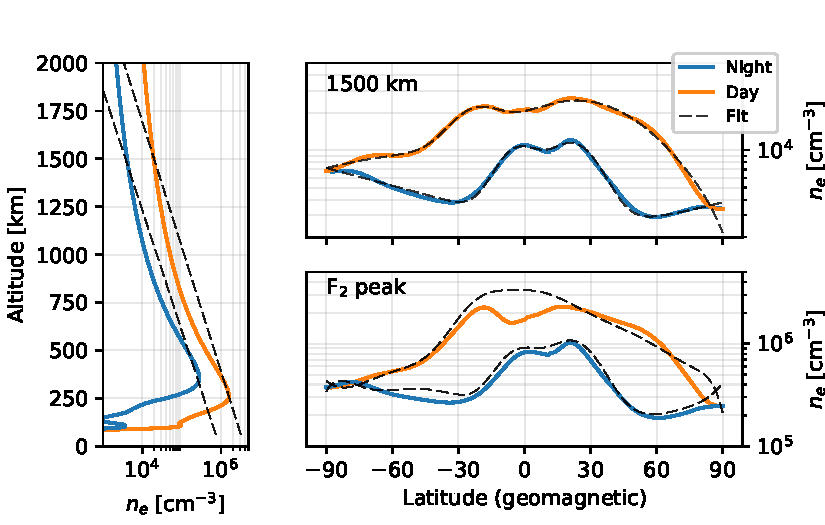
\includegraphics{figures/iono_profile.pdf}
\caption[Ionosphere density profile]{The IRI electron density model and derived curve fits. The left panel shows electron density variation as a function of altitude, for day and night. The right panels show electron density variation with respect to latitude, for 1500 km and the $F_2$ peak (approx. 300 km).}
\label{fig:iono_profile}
\end{center}
\end{figure}

In order to both reduce our model parameter space, and to greatly decrease computation time, we pair a simplified version of IRI with a simplified version of GCPM. The IRI-2016 model was run for dayside and nightside ionospheres (12 and 0 MLT), using all default settings, for January 1st, 2000. We then fit a multiple-Gaussian function to the electron density vs latitude, at an altitude of 1500 km, and at the $F_2$ peak. Electron density variation with respect to altitude is approximated by a log-linear fit between 1500 km and the $F_2$ peak. Finally, longitudinal variation is smoothed with a sigmoid function with a width of $\approx$ 1 hr. Figure \ref{fig:iono_profile} shows both the IRI electron density and the derived curve fits.


% RADIATION BELTS
